\documentclass[12p]{article}
\setlength{\parindent}{0em}
\usepackage{amsmath, mathrsfs, listings}
\usepackage{upquote, amssymb}
\usepackage[utf8]{inputenc}
\usepackage[english]{babel}
\usepackage[%
    left=0.50in,%
    right=0.50in,%
    top=1.0in,%
    bottom=1.0in%
]{geometry}%
\usepackage{graphicx}
\graphicspath{ {./images/} }
\renewcommand{\baselinestretch}{1.5}

\begin{document}

\section{(1) Adjon formulát abszolút folytonos eloszlású X valószínűségi változó esetén az Y = g(X) valószínűségi változó várható értékére!}

\section{(2) Legyen X standard normális eloszlású valószínűségi változó. Számítsa ki az X várható értékét! }

\section{(3) Mondja ki Bayes tételét. (3x)}

Legyen B1, B2, ..., pozitív valószínűségű eseményekből álló teljes eseményrendszer, A $\in$ $\mathscr{A}$ pozitív valószínűségű. Ekkor

$$\displaystyle{P(B_k|A) = \frac{P(A|B_k)P(B_k)}{\displaystyle{\sum_i} P(A|B_i)P(B_i)}}$$

\section{(4) Igazolja, hogy független azonos paraméterű binomiális eloszlású valószínűségi változók összege is ilyen.}

\section{(5) Írja fel az X és Y együttes eloszlásfüggvénye és az X perem eloszlásfüggvénye között fennálló kapcsolatot.}

\section{(6)  Definiálja a szórásnégyzetet és mondja ki legfontosabb tulajdonságait. (3x)}

$$D^2X = E[(X - E(X))^2] = EX^2 - E^2X$$

Tulajdonságok:

\begin{itemize}
	\item $D^2(X) \geq 0$, mert nemnegatív valószínőségi változó várható értéke
	\item $D^2(aX+b)=a^2D^2(X)$, mert $D^2(aX+b)=E[(aX+b-E(aX+b))^2]= E[(aX+b-aE(X)-b)^2]=E[(aX-aE(X))^2]=a^2 E[(X-E(X))^2]$.
	\item Abból, hogy $E(X)$ véges, még nem következik $D^2(X)$ végessége, hiszen ha $P(X=k)=c/k^3$ (egyértelmően megadható olyan c, amire ez eloszlás lesz) akkor $E(X)$ véges, de $E(X^2)=c(1+1/2+...+1/k...)$, ami végtelen.
\end{itemize}

\section{(7) Definiálja a konfidencia-intervallum fogalmát (3x)}

A konfidenciaintervallum a valószínűségi intervallum, az induktív statisztika eszköze: ha mintából becsülünk, sosem tudjuk a pontos értéket, a teljes sokaság felmérése igen drága dolog. A konfidenciaintervallum adott szignifikanciaszinten: a becsült változó alsó és felső korlátja.

(8) -

\section{(9) Adja meg a lineáris regresszió feladatát és megoldását.}

Az $Y = a_1X_1 + a_2X_2 + · · · + a_pX_p + b$ egyenletben az
együtthatók és a konstans meghatározása

Azaz:

$$\min_{a_1, ..., a_p,b} g(a_1,...,a_p,b) = \min_{a_1,...,a_p,b} E(Y - (a_1X_1 + ... + a_pX_p+b))^2$$

Megoldása:

b szerinti derivált:

$$\frac{\partial g}{\partial b} = -2E(Y - (a_1X_1 + ... + a_pX_p + b)) = 0$$

Kifejezve b-t:

$$b = EY - a_1EX_1 - ... - a_pEX_p$$

$a_i$ (i = 1, . . . , p) szerinti derivált:

$$\frac{\partial g}{\partial a_i} = -2E((Y-(a_1X_1 + ... + a_pX_p + b))X_i) = 0$$

b-t behelyettesítve az $a_i$ szerinti deriváltba:

\begin{align*}
0  &= -2E((Y - (a_1X_1 + ... + a_pX_p + b))X_i)\\
 &= -2E\left(\left((Y - EY) - \sum_{j = 1}^p a_j(X_j - EX_j)\right)X_i\right)\\
 &= -2(E(YX_i) - EYEX_i) +\\
 &+ 2 \sum_{j=1}^p a_j(E(X_iX_j) - EX_iEX_j)\\
 &= -2Cov(Y,X_i) + 2\sum_{j=1}^p a_j Cov(X_i,X_j), \quad i=1,...,p
\end{align*}

Jelölés: $C := Var(\underline{X})$, $d := Cov(Y, \underline{X})$
Ebből a következő egyenletrendszert kapjuk:
$$C\underline{a} = \underline{d}$$
melynek egyértelmű megoldása, ha C reguláris:
$$\underline{a} = C^{-1}\underline{d}$$
A második derivált vizsgálatával belátható, hogy ez
valóban minimum

\section{(10) Definiálja idősorok erős stacionaritását.}

Erős stacionaritás: az együttes eloszlások nem
függnek az időtől

\section{(11) Definiálja az ASN fogalmát.}

Az eljárás hatékonyságát mérő szám: várható mintaelemszám

$ASN = n_1 = n_2(1 - P^{I}_a - P^I_r)$, ahol $P_a^I$ annak valószínűsége, hogy az első minta alapján átvegyük a tételt, a $P_r^I$ pedig a visszautasítás valószínűsége.

\section{(12) írja fel az eloszás- és a sűrűségfüggvényeket karakterizáló tulajdonságokat! (3x)}

Eloszlásfüggvény:\\
$F_X(z):=P(X<z)$. $F_X(z):\mathbb{R}\rightarrow\mathbb{R}$ függvény az X valószínűségi változó eloszlásfüggvénye.\\
Tulajdonságai:

\begin{itemize}
	\item $0 \leq F_X(z) \leq 1$
	\item $F_X(z)$ monoton nő
	\item $\lim_{z \rightarrow \infty} F_X(z) = 1; \lim_{z \rightarrow -\infty} F_X(z) = 0$
	\item $F_X(z)$ balról folytonos
\end{itemize}

Sűrűségfüggvény:\\
Az X valószínűségi változó sűrűségfüggvénye $f(x) \leftrightarrow X$-re:

$F_X(z) = \int_{-\infty}^z f(t) dt$

Tulajdonságai:
\begin{itemize}
	\item $f \geq 0$
	\item $\int_{-\infty}^{\infty} f(t) dt = 1$
	\item Minden ilyen f integrálfüggvénye eloszlásfüggvény
\end{itemize}

\section{(13) Legyen X pascal eloszlású valószínűségi változó. Számítsa ki az X várható értékét!}

$$EX = \frac{1}{p}$$

\section{(14) Mi a kapcsolat az X és Y valószínűségi változó függetlensége és együttes eloszlásfüggvénye között? (3x)}

Független esetben az együttes eloszlásfüggvény a peremeloszlásfüggvények szorzatából kapható meg.

\section{(15) írja fel, az X diszkrét valószínűségi változó várható értékének definícióját! (2x)}

Egy X diszkrét valószínűségi változó (aminek az értékkészlete
$R_X$ és $i \in R_X$ esetén $P(X = i) = p_i)$ $E(X)$ várható értéke a lehetséges értékeinek a valószínűségekkel súlyozott átlaga, ha ez a sor abszolút konvergens.

$$E(X) = \sum_{i \in R_X} i * p_i$$

Ha a sor nem abszolút konvergens, akkor azt mondjuk, hogy nem létezik a várható érték.

(16) -

\section{(17) Vezesse le a polinomiális eloszlás koordinátái közötti korrelációra vonatkozó képletet.}

\section{(18) Definiálja a Poisson folyamatot. (3x)}

Poisson folyamat: időben lejátszódó folyamatnál adott [a,b) intervallumba eső események száma $(X_{a,b})$ éppen $\lambda(b-a)$ paraméterő Poisson eloszlású, ha a folyamat

\begin{itemize}
	\item homogén: $X_{a,a+t}$ eloszlása csak t-tıl függ;
	\item utóhatás nélküli: $X_{a,b}$ és $X_{b,c}$ függetlenek ha a<b<c;
	\item nemelfajuló: $0<P (X_{a,b}=0)<1$.

\end{itemize}

\section{(19) Mondja ki a nagy számok törvényének minél több változatát. (3x)}

	\subsection{Gyenge törvény}
	
	$X_1, X_2, ...$ függetlenek, azonos eloszlásúak, $EX_i = m < \infty$, $D^{2}X_i = \sigma^2 < \infty$. \\
	$P(\frac{X_1 + ... + X_n}{n} - m \geq \varepsilon) \rightarrow 0$ $(n \to \infty)$ $\forall \varepsilon > 0$-ra (sztochasztikus konvergencia).
	
	\subsection{Erős törvény}
	
	$X_1, X_2, ...$ függetlenek, azonos eloszlásúak, $EX_1 = m < \infty$, $D^{2}X_1 = \sigma^2 < \infty$. \\
	$\frac{X_1 + ... + X_n}{n} \rightarrow m$ $(n \to \infty)$ 1 valószínűséggel. \\
	Megjegyzés: Csebisev-egyenlőtlenséggel bizonyítjuk. ($\frac{\sigma^2}{n \varepsilon^2} \to 0$ $(n \to \infty)$)
	
	\subsubsection{Csebisev-egyenlőtlenség}
	
	$EX$ véges. \\
	Ekkor $P(|X-EX| \geq \lambda) \leq \frac{D^{2}X}{\lambda^2}$ \\
	Megjegyzés: Bizonyítás Markov-egyenlőtlenséggel.
	
	\subsubsection{Markov-egyenlőtlenség}
	
	$X \geq 0, c > 0$. \\
	Ekkor $P(X \geq c) \leq \frac{EX}{c}$
	


\section{(20) Vezesse le a Poisson eloszlás paraméterére a maximum likelihood becslést. (3x)}

Zyxon megoldasas:

A likelihood fuggveny:

$$L(\theta;\underline{x}) = f_{\theta}(\underline{x}) = \prod^n_{i=1} f_{\theta}(x_i)$$

Ennek maximumhelye lesz a $\theta$ paraméter maximum likelihood becslése. A Poisson-eloszlás paramétere: $\overline{X}$

Tankonyvar.hu-s megoldas:

$$P(X_1 = k) = \frac{\lambda^k}{k!}e^{-\lambda}\quad k=0, 1, 2, ...$$
A likelihood-fuggveny
$$L(x_1, ..., x_n;\lambda)=\prod^n_{i=1}\frac{\lambda^{x_i}}{x_i!}e^{-\lambda}$$
A loglikelihood-fuggveny
$$l(x_1, ..., x_n;\lambda) = \sum^n_{i=1}(x_i log \lambda - \lambda - log x_i!)$$
A maximumhelyet derivalassal hatarozzuk meg:
$$0 = \frac{\theta l(x_1, ..., x_n;\lambda)}{\theta \lambda} = \frac{1}{\lambda} \sum^n_{i=1} x_i - n$$
Innen
$$\hat{\lambda} = \frac{1}{n} \sum^n_{i=1} X_i = \overline{X}$$
A maximum-likelihood becsles.

\section{(21) Definiálja a lineáris modell hipotéziseit és adja meg a próbastatisztikát.}

\section{(22) Legyen X +1 és -1 értéket felvevő valószínűségi változó, $P(X = 1) = 1/6$ és $P(X = -1) = 5/6$. Számítsuk ki X várható értékét és szórás négyzetét.}

$$ E(X) = \frac{1}{6} * 1 + \frac{5}{6} * -1 = 2/3$$

$$ EX^2 = 1^2 * \frac{1}{6} + (-1)^2 * \frac{5}{6} = 1$$

$$ D^2(X) = EX^2 - E^2X = 1 - \left(\frac{2}{3}\right)^2 = \frac{5}{9}$$

\section{(23) Bizonyítsa be a nagy számok gyenge törvényét. (2x)}

\section{(24) Legyen $X^2$ egyenletes a $[0, 1]$-en. Adja meg X eloszlását és várható értékét.}

\section{(25) Irja fel a rendezett minta k-adik elemének a sűrűségfüggvényét.}

\section{(26) Rajzolja fel, hogyan lehet a sűrűségfüggvények segítségével a próbák kritikus értékeit és erőfüggvényüket szemléltetni!}

\section{(27) Definiálja a $\chi$-négyzet próbát és adja meg legfontosabb alkalmazásait.}

A Pearson-féle khí-négyzet ($\chi^2$) próba diszkrét eloszlású vagy ilyenné tehető változók vizsgálatára alkalmas statisztikai eljárás.

Illeszkedésvizsgálat $\displaystyle{\sum_{i=1}^r \frac{(v_i - np_i)^2}{np_i}}$\\
Homogenitásvizsgálat: $\displaystyle{nm \sum_{i=1}^r \frac{(\frac{v_i}{n}-\frac{\mu_i}{m})^2}{v_i + \mu_i}}$\\
Függetlenségvizsgálat: $\displaystyle{T_n = \sum_{i=1}^r \sum_{j=1}^s 
\frac{(v_{ij} - \frac{v_{i\cdot}v_{\cdot j}}{n})^2
}{\frac{v_{i\cdot}v_{\cdot j}}{n}}}$

\section{(28) Adja meg a lineáris regresszió feladatát és alkalmazásait.}

A statisztika eszköztárában a lineáris regresszió egy olyan paraméteres regressziós modell, mely feltételezi a magyarázó- (X) és a magyarázott (y) változó közti (paramétereiben) lineáris kapcsolatot. Ez azt jelenti, hogy lineáris regresszió becslése során a mintavételi adatok pontfelhőjére igyekszünk egyenest illeszteni.

Használható pl.:

\begin{itemize}
	\item Termékek árai és a vásárlási számok összefüggése
	\item Életkor és a halálozás kapcsolata
	\item Költség túllépési változók
\end{itemize}

\section{(29) Vezesse le a normális eloszlás várható értékére a momentum módszerrel adódó becslést.}

\section{(30) Adjon módszert idősorok simítására.}

Idősor simítása: kiszűri a rövidtávú ingadozások hatását,
eltünteti a szezonalitást

\begin{itemize}
	\item Mozgóátlag módszer
	\item Exponenciális simítás
\end{itemize}

(31) -

\section{(32) Mondja ki a centrális határeloszlás tételt. (2x)}

151.-es kerdesben benne van a valasz.

\section{(33) Legyen $X$ olyan valószínűségi változó, amely a (0, 1) intervallumból veszi fel az értékeit. Eloszlásfüggvénye ott F(t) = t/2 ha $t \in (0, 1/2]$, és $F(t) = 3/4 + t/4$ ha $t \in (1/2, 1]$. Rajzoljuk fel X eloszlásfüggvényét és számítsuk ki a $P(X \leq 1/2)$, valamint a $P(1/4 \leq X \leq 3/4)$ és $P(X = 1/2)$ valószínűségeket!}

\section{(34) Definiálja a teljes eseményrendszer fogalmát! (2x)}

Események $A_1, A_2, ...,$ sorozata teljes eseményrendszer, ha
egymást páronként kizárják és egyesítésük $\Omega$.

\section{(35) Definiálja a folytonos eloszlásokra a várható érték fogalmát.}

$$EX = \int_{-\infty}^{\infty} x f(x) dx$$
ha az integral letezik.

\section{(36) Mondja ki Bernstein tételét.}

Legyen $(X_1, X_2, ..., X_n)$ olyan, hogy $D^2(X_1) + D^2(X_2) ... + D^2(X_n) < kn$, valamint tegyük fel, hogy van olyan $h: N \rightarrow R_{+}$ függvény, melyre $|R(X_i, X_j)| \leq h(|i-j|)$ és $\frac{1}{n} \displaystyle{\sum^n_{i=1}} h(i) \rightarrow 0$ ekkor $(X_1 + ... + X_n) / n - (m_1 + m_2 + ... + m_n)/n \rightarrow 0$ sztohasztikusan.

\section{(37) Bizonyítsa be a Markov egyenlőtlenség általános alakját.}

77.-es kerdesben!

\section{(38) Definiálja a maximum-likelihood módszert.}

Azt a paraméterértéket keressük, ahol a likelihood függvény a legnagyobb értéket veszi fel (azaz diszkrét esetben az
ismeretlen paraméter azon értéket keressük, amely mellett a bekövetkezett eredmény maximális valószínűségű): $\max_{\theta}L(\theta; x)$.

Ez nyilván megegyezik azzal a paraméterértékkel, ahol a log-likelihood függvény veszi fel a legnagyobb
értéket, azaz: $\max_{\theta} l(\theta; x)$.

Amennyiben a függvény deriválható $\theta$ szerint, akkor a maximumot kereshetjük a szokásos módon, a deriváltak
segítségével, azonban a feladatunkat jelentősen megnehezíti, hogy olyan n-szeres szorzatot kellene deriválni, amelyiknek minden tagjában ott van az a változó, ami szerint deriválnunk kellene. Ezért likelihood függvény helyett a log-likelihood függvény maximumhelyét keressük.

Ha $\theta$ 1 dimenziós, akkor $\partial_\theta l(\theta, x) = 0$, míg ha $\theta = (\theta_1, ..., \theta_p)$ p dimenziós, akkor $\partial_{\theta_i} l(\theta, x) = 0$ megoldásából
kapjuk a becslést. (A második deriváltak segítségével ellen ˝orizz¨uk, hogy valóban maximum.)


\section{(39) Definiálja a Wilcoxon próbált.}

Ez a próba olyan kísérleti helyzetekben alkalmazható, ahol a mintavétel a páros megfigyelésen alapul, ahol 2 összefüggő változóból mintavétel történik, úgy, hogy mindegyikből egy-egy jut egy megfigyelési egységbe.

A próba feltételei:
\begin{itemize}
	\item Ordinális skálán mérhető folytonos valószínűségi változók esetén akkor alkalmazható,
	\item ha a különbségek is ordinális skálán mérhetőek.
	\item Erősen asszimmetrikus eloszlás esetén nem alkalmazható.
\end{itemize}

\section{(40) Definiálja az autoregressziós és a mozgóátlag folyamatokat.}

Autoregresszív folyamat

Az $Y_t$ diszkrét paraméterű sztochasztikus
folyamatok k-ad rendű autoregresszív
folyamatnak nevezzük, ha

$$Y_t = \alpha_1 * Y_{t-1} + \cdots + \alpha_k * Y_{t-k} + \mathcal{E}_t$$

Ahol:\\
$\alpha_i$ konstansok\\
$Y_t$ fehér zaj (várható értéke 0, szórása $\sigma_y$)

Mozgóátlag-folyamat

Az $Y_t$ diszkrét paraméterű sztochasztikus
folyamatot k-ad rendű mozgóátlag folyamatnak
nevezzük, ha

$$Y_t = \beta_0 * U_t + \beta_1 * U_{t-1} + \cdots + \beta_k * U_{t-k}$$

Ahol\\
$\beta_k$ konstansok\\
$U_t$ diszkrét fehér zaj (várható érték 0, szórás $\sigma_u$)

\section{(41) Mit jelent a becsléses illeszkedésvizsgálat és hogyan alkalmazzuk rá a $\chi$-négyzet próbát?}

Legyen $\theta$ egy $s$ dimenziós paramétervektor, valamint legyen $\hat{\theta}$ a $\theta$ paramétervektor ML-becslése, és legyen $\hat{p}_j = p_j(\hat{\theta})$

$H_0 : P(X_i = x_j) = \hat{p}_j \quad j=1,\cdots,r$\\
$H_1 : \exists$ legalább egy j melyre $P(X_i = x_j) \neq \hat{p}_j$\\
Próbastatisztika: $$T_n = \sum^r_{j=1} \frac{(v_j - n\hat{p})_j)^2}{n\hat{p}_j} \stackrel{H_0 eseten}{\sim} \chi^2_{r-s-1}$$
Kritikus tartomány: $$\chi_k = \{x: T_n(x) > \chi^2_{r-s-1,1-\alpha}\}$$

\section{(42) Legyen X n-edrendű p paraméterű binomiális eloszlású valószínűségi változó. Számítsa ki az X várható értékét!}

$$EX = np$$

\section{(43) Mondja ki a szita (Poincaré) formulát.}

Képlet az általános esetre:

$$P(A_1 \cup A_2 \cup ... \cup A_n) = \sum^n_{i=1} (-1)^{i+1} S^{(n)}_i$$
ahol
$$S^{(n)}_i = \sum_{1 \leq j_1 < j_2 < ... < j_i \leq n} P(A_{j_1}, \cap A_{j_2} \cap ... \cap A_{j_i})$$

az i tényezıs metszetek
valószínőségeinek összege.

\section{(44) Definiálja a kovarianciát és írja le tulajdonságait. (4x)}

$cov(X,Y) := E[(X-E(X))(Y-E(Y))]$

Kiszámítása:
$cov(X,Y) = E(XY)-E(X)E(Y)$

Ha X és Y függetlenek $\rightarrow$ $cov(X,Y) = 0$, fordítva nem feltétlenül igaz

A kovariancia szimmetrikus: $cov(X,Y) = cov(Y,X)$

$cov(X,X) = D^2(X)$

\section{(45) Mondja ki a centrális határeloszlás tétel lokális változatát. (2x)}

Legyenek $X_1 , X_2 ,..., X_n ,...$ független, azonos eloszlású, abszolút folytonos valószínőségi változók. Tegyük fel, hogy $\sigma_2=D_2(X)$ véges $(m:=E(Xi))$ és hogy $f(x)$ korlátos. Tekintsük a standardizált összegüket:

$$Z_n := \frac{X_1 + ... + X_n - nm}{\sqrt{n}\sigma}$$

Ekkor $Z_n$ sűrűségfüggvénye konvergál a standard normális
eloszlás sőrőségfüggvényéhez, azaz

$$\lim_{n \rightarrow \infty} f_n(x) = \frac{1}{\sqrt{2\pi}} e^{- \frac{x^2}{2}}$$

A konvergencia z-ben egyenletes.

\section{(46) Legyen X egyenletes a [0,1]-en. Adja meg $X^2$ eloszlását és várható értékét.}

\section{(47) Irja fel a Nadarajah módszer lényegét és szemléltesse grafikusan az eljárás motivációját! }

Ha csak mért adataink vannak, közelítjük a
feltételes várható értéket (hasonló a ParzenRosenblatt becsléshez).

$$\hat{r}_n(x) = \frac{\displaystyle{\sum^n_{i=1} Y_ik \left(\frac{x - X_i}{h_n}\right)}}{\displaystyle{\sum^n_{i=1} k \left(\frac{x - X_i}{h_n}\right)}}$$

A Parzen-Rosenblatt tétel feltételei esetén ez
konzisztens becslése az E(Y|X) regressziónak.

\section{(48) Definiálja a 2 mintás t-próbát és vezesse le a próbastatisztika képletét!}

\textit{t-próba}:	Ennél a próbánál nem ismert a szórás, viszont ugyanúgy normális eloszlást feltételezünk, mint az u-próbánál. $\xi_i \sim N(m, \sigma^2)$, $i=1..n$.

\textit{Kétmintás}: $\xi_i \sim N(m_1, \sigma_1^2)$, $i=1..n$ és $\eta_j \sim N(m_2, \sigma_2^2)$, $j=1..m$. Ez esetben sem ismert a szórás, viszont feltételezzük, hogy a két minta szórása megegyezik. Ekkor 
$$\displaystyle{t = \sqrt{\frac{nm}{n+m}}\frac{\overline{X} - \overline{Y}}{\sqrt{\frac{(n-1)(s^*_1)^2 + (m-1)(s^*_2)^2}{n+m-2}}} \stackrel{H_0 eseten}{\sim}
t_{n+m-2}}$$
$n+m-2$ a próba szabadságfoka.

\section{(49) Mondja ki a Neyman-Pearson lemmát!}

A próba legerısebb a saját terjedelmével. Minden legerısebb próba ilyen alakú

\section{(50) Definiálja az autokorrelációs együtthatókat és adja meg becslésüket arra az esetre, amikor reziduálisokból számolunk!}

\section{(51) Definiálja a valószínűségi mező fogalmát! (2x)}

($\Omega, \mathcal{A}, P$) Kolmogorov-féle
valószínűségi mező, ha
\begin{itemize}
	\item $\Omega$ nemüres halmaz
	\item $\mathcal{A}$ az $\Omega$ részhalmazainak $\sigma$-algebrája
	\item $P: \mathcal{A} \rightarrow [0, 1]$  halmazfüggvény
(valószínűség) , melyre
	\item $P(\Omega) = 1$
	\item $\sigma$-additivitás: ha $A_1, A_2,\cdots,$ páronként
kizáró események, akkor $P(A_1 \cup A_2 \cup \cdots) = P(A_1) + P(A_2) + \cdots$
\end{itemize}

\section{(52) Vezesse le, hogy a korrigált tapasztalati szórásnégyzet torzítatlan becslés a szórásnégyzetre. }

\section{(53) Vezesse le, hogy a relatív gyakoriság konzisztens becslés a valószínűségre.}

\section{(54) Definiálja becslések aszimptotikus torzítatlanságát.}

$T_n(X)$ a $\theta$ paraméter konzisztens becslése, ha
$$E_{\theta}(T_n(\underline{X})) \rightarrow \theta$$

\section{(55) Definiálja a t-próbát az egy- és kétmintás esetre is.}


Egymintás
$\sigma$ ismeretlen; Probastatisztika:

$$T(X) = t = \frac{\overline{X} - m_0}{\frac{s^{*}_n}{\sqrt{n}}} \stackrel{H_0 eseten}{\sim} t_{n-1}$$

Kritikus tartományok:

$$\chi_k = \{X: |t| > t_{n-1,1-\alpha/2}\} \quad \chi_k = \{X: t > t_{n-1,1-\alpha}\} \quad \chi_k = \{X: t < t_{n-1, \alpha}\}$$

Kétmintás

Probastatisztika:

$$\displaystyle{t = \sqrt{\frac{nm}{n+m}}\frac{\overline{X} - \overline{Y}}{\sqrt{\frac{(n-1)(s^*_1)^2 + (m-1)(s^*_2)^2}{n+m-2}}} \stackrel{H_0 eseten}{\sim}
t_{n+m-2}}$$

\section{(56) Definiálja a szekvenciális próbát (egyszerű hipotézisek esetére).}

A valószínőséghányados n elemő mintából

$$\displaystyle{V_n = \frac{\prod^n_{i=1} f_1(X_i)}{\prod^n_{i=1} f_0(X_i)}}$$

\begin{itemize}
\item Addig veszünk mintaelemeket, amíg $V_n \geq B$ vagy $V_n \leq A$ nem teljesül\\
Tehát az algoritmus:
\item $V_n \geq B$: elutasítjuk $H_0$-t
\item $V_n \leq A$ : elfogadjuk $H_0$-t.
\item $B>Vn>A$: új mintaelemet veszünk.
\end{itemize}

\section{(57) Definiálja a korrelációs együtthatót és mondja ki legfontosabb tulajdonságait.}

A változók közötti lineáris kapcsolat erősségét mérő
mennyiség a korrelációs együttható: 

$$R(X, Y) = \frac{cov(X,Y)}{D(X)D(Y)}$$

Tulajdonságai:

\begin{itemize}
\item $R(X,Y)=0$, ha X és Y függetlenek (ez sem
fordítható meg)
\item Ez alapján definíció szerint legyen R(X,Y)=0, ha X
vagy Y elfajult eloszlású.
\item $R(X,aX+b)=1$, ha $a>0$, mert $cov(X,aX+b)=aD^2(X)$
\end{itemize}


\section{(58) Mikor nevezünk egy torzítatlan becslést hatásosabbnak egy másiknál?}

$T_1$ hatásosabb becslése a $\theta$ paraméternek a $T_2$-nél, ha
$$D_{\theta}^2(T_1(\underline{X})) \leq D_{\theta}^2(T_2(\underline{X}))$$
teljesül minden $\theta$ paraméterértékre.

\section{(59) Definiálja idősorokra a trend és a periódus fogalmát.}

Különböző, eltérő tartalmú
komponensekre bontott idősor, additív vagy multiplikatív
formában felépítve. Pl.: additív esetben

$$Y_t = T_t + C_t + S_t + u_t$$

ahol T, C és S a trend, a ciklikus és a periodikus komponens,
u pedig a véletlen folyamat.

\section{(60) Adjon példát olyan maximum likelihood becslésre, ami nem torzítatlan! (3x)}



\section{(62) Definiálja valószínűségi változók eloszlását.}

Mivel a gyakorlati problémáknál $\Omega$ nem
mindig adható meg egyértelműen, és
absztrakt halmazok helyett szívesebben
dolgozunk a valós számokkal, a kulcsfogalom
a valószínűségi változók eloszlása.\\
Legyen B tetszőleges Borel halmaz.
$Q_X(B):= P{\omega: X(\omega) \in B}$ valószínűséget ad
meg R Borel halmazain. Ez az X eloszlása.\\

\section{(63) Mit jelent a valószínűség folytonossága?}

Ha $A_i \in \mathcal{A} (i = 1,2,\cdots)$ és $A_1 \supseteqq A_2 \supseteqq \cdots$ akkor az $\displaystyle{A = \cap^{\infty}_{i=1}A_i}$ jelöléssel $\lim_{n \rightarrow \infty} P(A_n)=P(A)$

\section{(64) Definiálja n valószínűségi változó függetlenségét.}

 Az $X_1,...,X_n$ valószínűségi változók függetlenek, ha az $\mathscr{F}_{X1}, \mathscr{F}_{X2} ,...,\mathscr{F}_{X_n}$ generált $\sigma$-algebrák függetlenek.

\section{(65) Definiálja diszkrét valószínűségi változók együttes eloszlását!}

az X diszkrét valószínűségi változó, ha értékkészlete $(x_1 ,..., x_n...)$ legfeljebb megszámlálható.\\
A valószínűségi változó definíciójából adódóan $\{\omega:X(\omega)= x_i\}=\{X=x_i\}= \in \mathscr{A}$ azaz $p_i:=P$ $(X=x_i)$értelmes. Ezek meg is határozzák X eloszlását.

\section{(66) Definiálja a t eloszlást!}

Definíció:  Az X  valószínűségi változót $n$ szabadságfokú Student eloszlásúnak nevezzük, ha sűrűségfüggvénye:

$$f(x) = \frac{\Gamma \left(\frac{n+1}{2}\right)}{\sqrt{\pi} \sqrt{n \Gamma} \left(\frac{n}{2}\right) \left(1 + \frac{x^2}{n}\right)^{\frac{n+1}{2}}}$$

\section{(67) Definiálja a gyenge konvergenciát!}

$P_n \rightarrow P$ gyengén, ha minden $f: S \rightarrow R$ folytonos, korlátos függvényre

$$\int fdP_n \rightarrow \int fdP$$

Tulajdonságok: többek között azzal is
ekvivalens, hogy $P_n(A) \rightarrow P(A)$ minden P-folytonossági halmazra.

\section{(68) Irja fel annak a valószínűségét, hogy a 90/5-ös lottónál egy szelvénnyel játszva legalább 2 találatunk lesz!}

\section{(69) Legyen az alábbi 3 megfigyelésünk az $(X, Y)$ párra. $(1;2)$ $(1.2;2.5)$ $(0.8;1.6)$. Nadarajah
módszerét használva a $k(x) = 1$, ha $-1/2 < x < 1/2$ (és 0 különben) magfüggvénnyel és a $h = 0.5$ ablakszélességel, mi lesz az $E(Y|X = 1.1)$ becslése?}

\section{(70) Vezesse le egyszerű hipotézisekre, hogy az egymintás u-próba valószínűséghányadospróba az egyoldali ellenhipotézis esetén!}

\section{(71) Hogyan tudjuk a lineáris modellt alkalmazni polinommal történő közelítésre?}

\section{(72) Adjon példát olyan maximum likelihood becslésre, mely nem torzítatlan.}

\section{(73) Definiálja az előjelpróbát! Mik a kritikus értékek? (3x)}

Nemparaméteres próba, illeszkedésvizsgálat $\rightarrow$ adott eloszlású-e a minta?

Az előjelpróba a különbségek előjelén alapul. $H_0$ esetén Binom(n; 1/2).

\section{(74) Adjon példát olyan $X_n$ valószínűségi változó-sorozatra, amely független tagú, de mégsem teljesül rá a centrális határeloszlástétel.}

\section{(75) Legyen X egyenletes eloszlású a [-1, 1] intervallumon. Számítsa ki $X^2$ sűrűségfüggvényét.}

\section{(76) Definiálja a normális eloszlást és vezesse le a legfontosabb tulajdonságait.}

Feltűnő tulajdonsága a normális eloszlásnak, hogy nem ferde, illetve az átlagra szimmetrikus. Ez azt jelenti, hogy a normális eloszlás átlaga, mediánja és módusza egyenlő. A normális eloszlás alakját haranghoz szokás hasonlítani.

$N(m, \sigma^2)$; Eloszlasfuggveny: visszavezetheto $\Phi$-re\\ Surusegfuggveny: $$\displaystyle{\frac{1}{\sqrt{2\pi} \sigma}e^{-\frac{(x-m)^2}{2\sigma^2}}}$$

EX: m\\
$D^2X: \sigma^2$

\section{(77) Mondja ki és bizonyítsa is be a Markov egyenlotlegnséget.}

Legyen $g : \mathbb{R} \rightarrow \mathbb{R}$ monoton növő pozitív függvény, $X \geq 0$ valószínűségi változó, melyre $EX < \infty$ és $\mathcal{E} > 0$ tetszőleges. Ekkor

$$P(X \geq \mathcal{E}) \leq \frac{E(g(X))}{g(\mathcal{E})}$$

Spec., ha $g(x) = x$, akkor

$$P(X \geq \mathcal{E}) \leq \frac{EX}{\mathcal{E}}$$

Bizonyitas diszkret esetre

$$E(X) = \sum_{i \in R_X} i*p_i = \sum_{i>0,i\in R_X} i*p_i \geq \sum_{i \geq a, i\in R_X} i*p_i \geq \sum_{i\geq a, i\in R_X} a*p_i = aP(X \geq a)$$

Bizonyitas folytonos esetre

$$E(X) = \int_{-\infty}^{\infty} yf_X(y)dy = \int_{0}^{\infty} yf_X(y)dy \geq \int_{a}^{\infty} yf_X(y)dy$$
$$\int_{a}^{\infty}yf_X(y)dy \geq \int_{a}^{\infty} af_X(y)dy = a * P(X \geq a)$$

\section{(78) Hogyan alkalmazhatjuk a Kolmogorov-Szmirnov próbát véletlenszám-generátorok tesztelésére?}

A tapasztalati és az elméleti eloszlásfüggvény
legnagyobb eltéréseit karakterizálja

$$K_n^{+} = \sqrt{n} \max (F_n(x) - F(x)), \quad K_n^{-}=\sqrt{n} \max(F(x) - F_n(x))$$

Táblázatból kiolvasható a keresett valószínűség\\
A kis lokális eltéréseket nem mutatja ki

\section{(79) Definiálja a binomiális eloszlást, vezesse le a képletét és adja meg alkalmazási lehetőségeit!}

\subsection{Levezetes}

Amennyiben N úgy tart a végtelenhez, hogy közben $M/N \rightarrow p$ (ahol $p \in (0,1)$), akkor a hipergeometrikus eloszlás tart a binomiális eloszláshoz:

$$\lim_{N \rightarrow \infty, N/M \rightarrow p} {M \choose k}{{N - M} \choose {n - k}}/{N \choose n} = {n \choose k}p^k(1-p)^{n-k}$$

\subsection{Alkalmazas}
\begin{itemize}
\item Visszatevéses mintavétel más realizációja: független kísérletek azonos körülmények között. $P(A) = p$ esemény, végezzünk n(rögzített számú) független kísérletet.
\item X: az A bekövetkezésének gyakorisága (pontosan hányszor jött ki az A). X eloszlása binomiális (n,p).
\item $X = X_1 + X_2 + \cdots + X_n$ ahol $X_i$ az i-edik kísérletnél az A esemény indikátora. Ezek az indikátorok függetlenek is!

\end{itemize}

\section{(80) Legyenek az adataink: 1,2,5,6. Számolja ki a mediánt és rajzolja fel a tapasztalati eloszlásfüggvényt!}

\section{(81) Tegyük fel, hogy egy 10 fős csoportban mindenki kihúzza valakinek a nevét a karácsonyi ajándékozásnál. várható értékben hány ember húzta saját magát? Vezesse is le az eredményt!}

\section{(82) Rajzolja fel a $\lambda = 1$ és $\lambda = 2$ paraméterű exponenciális eloszlás sűrűség- és eloszlásfüggvényét!}

\section{(83) Vezesse le a $[0, \theta]$ intervallumon egyenletes eloszlásra a maximum likelihood becslést n mintaelem alapján!}

\section{(84) Rajzolja fel az alábbi minta tapasztalati eloszlásfüggvényét: 1,5,6,7! (2x)}

\section{(85) Hogyan tudunk inverz módszerrel véletlen számot generálni? (2x)}

Legyen X val. vált., F eloszlásfüggvénnyel,
amely monoton növekedı és folytonos. Ekkor

\begin{itemize}
	\item F(X) egyenetes eloszlású [0, 1]-en.
	\item Ha $U \sim U(0, 1)$ akkor $F^{-1}(U)$ eloszlásfüggvénye F.
\end{itemize}

Pl.:

$$X \sim exp(\lambda) \rightarrow F(x) = 1-exp(-\lambda x) \rightarrow F^{-1}(x) = -\ln (1-x)/\lambda \rightarrow -\ln(1-U)/\lambda \sim exp(\lambda)$$

\section{(86) Legyen az X valószínűségi változó sűrűségfüggvénye $f(x) = x^2/9$, ha $0 < x < 3$ és $0$ különben. Adjuk meg $X$ eloszlásfüggvényének értékét az $1/2$ helyen. $E(1/X)=?$ Adjuk meg $sqrt{X}$ sűrűségfüggvényének értékét az $1/2$ helyen.}

\section{(87) Számítsa ki annak a valószínűségét, hogy egy háromgyerekes családban azonos neműek a gyerekek! (Tegyük fel, hogy a fiúk és lányok szóletési valószínűsége is 0.5 és hogy az egyes születések függetlenek.)}

\section{(88) Definiálja a várható érték fogalmát diszkrét valószínűségi változókra!}

A $p_i =P (X=x_i)$ eloszlással megadott valószínőségi változó várható értéke $E(X):= p_1x_1+ p_2x_2 +...,$ ha a sor abszolút konvergens.

\section{(89)  Legyen X egyenletes eloszlású a $[-2,2]$ intervallumon. Adja meg $(X - 2)(X + 2)$ sűrűségfüggvényét.}

\section{(90) Mondja ki abszolút folytonos valószínűségi változók függetlenségének ekvivalens jellemzőit. (2x)}

Ha X koordinátái függetlenek, akkor definíció szerint:

$F_X(z) = P(X_1<z_1, X_2<z_2, ..., X_d<z_d) = F_1(z_1)F_2(z_2)...F_n(z_n) \forall z \in \mathbb{R}^d$

\section{(91) Mondjon példát az egyenletes, az exponenciális és a normális eloszlás alkalmazására!}

Egyenletes eloszlás:\\
Véletlengenerátorokban igyekeznek az egyenletes eloszlást egy adott intervallumon minél inkább közelíteni

Exponenciális eloszlás:\\
Előrejelzéseknél alkalmazzák: n adatpontos minta megfigyelése után egy ismeretlen exponenciális eloszlású forrásból meg tudjuk jósolni, hogy mi lesz a következő érték ugyanabból az ismeretlen exponenciális eloszlású adatforrásból

Normális eloszlás:\\
Mérési hibákra, mért ingadozásokra és olyan élettartam vizsgálatokra használjuk, ahol a készülékek, alkatrészek rendszeres kopással mennek tönkre. Bizonyos feltételek eseték a binomiális eloszlás közelítésére is használható.

\section{(92) Definiálja a bootstrap módszert.}

\begin{itemize}
	\item Adott $X_n$-ből m elemű visszatevéses mintát veszünk (általában m=n) \quad $X^{*}_m = \{X^{*}_1,...,X^{*}_m\}$
	\item $X_i^{*}$ közös eloszlása: $F_n = n^{-1} \sum^n_{i=1} \delta_{x_i}$
	\item $T^{*}_{m,n} = t_m (X^{*}_m;F_n)$
	\item Ismétlés $\rightarrow \hat{G}_{m,n}$
	
\end{itemize}


\section{(93) Mi a leíró statisztika feladata?}

Célja egy már rendelkezésre álló, valóságra vonatkozó adathalmaz összefoglalása, elemzése, egyszóval az információtömörítés.\\

\section{(94) Definiálja a kovarianciát!}

$$cov(X, Y) = E(XY) - EXEY$$

\section{(95) Mihez tart $P(X1+X2+ ... +Xn > 9n/2)$, ha $X1, X2, . . .$ független, a $[4,6]$ intervallumon
egyenletes eloszlású valószínűségi változók és n tart végtelenhez?}

\section{(96) Vezesse le az exponenciális eloszlás várható értékére vonatkozó képletet!}

$$E \xi = \int^{\infty}_0 x \cdot \lambda \cdot e^{-\lambda x} dx = [-x \cdot e^{-\lambda x}]^{\infty}_0 + \int^{\infty}_0 e^{-\lambda x} dx = \left[\frac{e^{-\lambda x}}{-\lambda} \right]^{\infty}_0 = \frac{1}{\lambda}$$

\section{(97) Legyen az alábbi 3 megfigyelésünk az $(X, Y)$ párra. $(1;2)$ $(1.3;2.5)$ $(0.8;1.5)$. Nadarajah
módszerét használva a a $k(x) = 1$, ha $-1/2 < x < 1/2$ (és 0 különben) magfüggvénnyel és a $h = 0.5$ ablakszélességgel, adjon becslést $Y$ közelítésére, ha $X = 1$.}

\section{(99) Az alábbi minta: 0,0,1,1,2 alapján becsüljük torzítatlanul az alábbi paramétereket:
várható érték, szórásnégyzet, annak a valószínűsége, hogy $X > 0.2$.}

\section{(100) Adjon módszert arra, hogyan szimulálna véletlen számot a $\sin x (0 < x < \pi/2)$ sűrűségfüggvényű eloszlásból!}

\section{(101) Hogy hívjuk a $h(t) = E(|X - t|^2)$ függvény minimum helyét?}

\section{(102) Hogyan adhatjuk meg a megszámlálható valószínűségi mezőn a valószínűséget?}

$$P(A) = P(\cup_{i:\omega_i \in A} \omega_i) = \sum_{i:\omega_i \in A} p_i$$

\section{(103) Legyen X 5 várható értékű és 2 szórású normális eloszlású, Y pedig az X = 7 esemény indikátora. Számítsa ki Y várható értékét és szórását!}

\section{(104)  Definiálja a visszatevés nélküli mintavétel modelljét és adja meg a különböző selejtszámok valószínűségeit!}

N termék, melyből M selejtes\\
n elemő minta visszatevés nélkül\\
A: pontosan k selejtes van a mintában
(k=0,...,n)

$$P(A) = \frac{{M \choose k}{{N - M} \choose {n - k}}}{{N \choose n}}$$

\section{(105) Mondja ki a Markov egyenlőtlenséget!}

77.-es kerdesben!

\section{(106) Vezesse le a valószínűségre a maximum likelihood becslést n mintaelem alapján!}

\section{(107) Definiálja a sztochasztikus konvergenciát! (2x)}

 minden $\mathcal{E}$, $\delta>0$-
hoz megadható olyan $n_0$, hogy $n>n_0$ esetén $P(|X_n-X| \geq \mathcal{E}) \leq \delta$.

Lemma

$$X_n \rightarrow X m.m. \leftrightarrow \lim_{m \rightarrow \infty} P(\sup_{n \geq m} |X_n - X| > \mathcal{E}) = 0$$

Köv.: A m.m. konvergenciából következik a
sztochasztikus konvergencia.


\section{(108) Írja le a sűrűségfüggvény becslésére tanult eljárást.}

$$f_n(x) = \frac{1}{nh_n}\sum^n_{i=1}k\left( \frac{x-X_i}{h_n} \right)$$

\section{(109) Adja meg a legkisebb négyzetes becslést a lineáris modellben. Mik a tulajdonságai?}

\section{(110) Legyen X egyenletes a $[0, 1]$-en. Adja meg $X^2$ eloszlását és várható értékét.}

\section{(111) Számolja ki a Wilcoxon próbastatisztika értékét az alábbi két adatsorra! Hogyan döntene arról, hogy tekinthetők-e azonos eloszlásból származónak? Az első minta: 1,2,4,12,23,50;
a második minta: 3,8,15,25,61,200.}

\section{(112) Definiálja az F-próbát és adja meg legfontosabb alkalmazásait. (2x)}

$$H_0: \sigma_1 = \sigma_2$$
$$H_1: \sigma_1 \neq \sigma_2$$
Probastatisztika
$$F= \frac{(s_1^{*})^2}{(s_2^{*})^2} \stackrel{H_0 eseten}{\sim} F_{n-1,m-1}$$

\section{(113)  Hogyan generálhatunk véletlen számot Neumann módszerével?}

Legyen f(x) tetszőleges sűrűségfüggvény, $g(x)$ pedig olyan sűrűségfüggvény, amelyre $f(x) < Mg(x)$, valamely $M>1$ esetén és $g(x)$-ből könnyen tudunk mintát venni (tipikus példa az egyenletes eloszlás).

\section{(114) Töltse ki az alábbi táblázat hiányzó celláit úgy, hogy a peremeloszlások egyenletesek
legyenek a megadott számokon! Függetlenek-e ezek a változók? Számolja ki az $E(X^2Y)$ várható értéket!}

\begin{center}
 \begin{tabular}{| c c || c | c | c | c |} 
 \hline
 Y & X &  0 & 1 & 2 & 3\\ [0.5ex] 
 \hline\hline
 0 &  & 0,2 & & 0,05 & \\ 
 \hline
 1 &  & & 0,15 & & \\
 \hline\hline
\end{tabular}
\end{center}

\section{(115) Mutassa meg, hogy független azonos paraméterű binomiálisok összege binomiális eloszlású! Mi a kapcsolat a rendek között?}

\section{(116) Definiálja két esemény függetlenségét!}

Az A és B események függetlenek, ha $P(A \cap B) = P(A)P(B)$.

\section{(117) Számítsa ki két kockadobás maximumának a várható értékét.}

\section{(118) Definiálja az első- és másodfajú hiba fogalmát, valamint próbák konzisztenciáját.}

Első:\\
Valamely nullhipotézis statisztikai próbával végzett vizsgálatában az a hiba, amelyet a nullhipotézis elutasítása jelent amikor az igaz. Valószínûsége az elsõfajú kockázat (alfa). 

Másodfajú hiba\\
Az a hibás döntés, hogy nem vetjük el a helytelen nullhipotézist abban az esetben, amikor az alternatív hipotézis igaz. A próba közvetlenül nem ellenõrzi, ezért ha a próba nem utasítja el a nullhipotézist, ez még nem jelenti azt, hogy a nullhipotézist megfelelõ statisztikai biztonsággal elfogadhatjuk. Valószínûsége a másodfajú kockázat (béta). 

Konzisztencia\\
Az erőfv. 1-hez tart (minden $\theta \in \Theta_1-re$)


\section{(119) Irja le a t-próba alkalmazását a párosított megfigyelések esetére.}

Példa: Van-e különbség Budapest és Cegléd napi átlaghımérséklete között?$H_0: m_1=m_2$ a nullhipotézis. 

Ha ugyanazon napokról van megfigyelésünk
mindkét helyen: nem függetlenek a minták.
Ekkor a párok tagjai közötti különbséget
vizsgálva, az előző egymintás esetre
vezethetı vissza a feladat. $H_0*: m=0 ,H_1^{*}:m\neq0$ az új hipotézisek. 


\section{(120) Vajon van-e stacionárius megoldása az $X_n = 0.96 X_{n-1} + \epsilon_n$ rekurziónak? Válaszát
indokolja!}

\section{(121) Legyen a mintaelemek sűrűségfüggvénye $f(x) = (\theta + 1)x^{\theta}$ ha $0 < x < 1$ ($\theta \geq$ 0 a par.).
Egy mintaelem alapján határozzuk meg az $\alpha = 0.05$ terjedelmű valószínűséghányadospróbát a $H_0 : \theta = 0, H_1 : \theta = 1$ hipotézisekre!}

\section{(122) Ismertesse a lineáris regresszió együtthatóira vonatkozó próbák lényegét! (2x)}

??

\section{(123) Adott n elemű minta az alábbi eloszlásból: $P(Z = 1) = c$, $P(Z = 2) = 2c$, $P(Z = 3) = 1 - 3c$ ($0 < c < 1/3$ az ismeretlen paraméter). Határozza meg a paraméter maximum likelihood becslését!}

\section{(124) Számítsa ki két kockadobás minimumának a várható értékét.}

\section{(125) Írja fel a Csebisev egyenlőtlenséget, és vázolja a bizonyítását.}

Legyen X tetszőleges valószínűségi változó, melyre $D^2X < \infty$ és $\mathcal{E} > 0$ tetszőleges. Ekkor

$$P(|X - EX| \geq \mathcal{E}) \leq \frac{D^X}{\mathcal{E}^2}$$

Bizonyítás:

Az $Y = |X - E(X)|$ valószínűségi változóra írjuk fel a Markov-egyenlőtlenség erősebb formáját.

$$g(a)P(|X - E(X)| \geq \mathcal{E}) \leq E(g(|X - E(X)|))$$

Ekkor ha a $g(x) = x^2$, ha $x > 0$, egyébként 0 függvényt írjuk be (ami monoton növő):

$$\mathcal{E}^2P(|X - E(X)| \geq \mathcal{E}) \leq E((|X - E(X)|)^2) = E((X - E(X))^2) = D^2(X)$$

\section{(126) Legyen X 5 várható értékű Poisson eloszlású, Y pedig az X = 5 esemény indikátora. Számítsa ki Y várható értékét és szórását!}

\section{(127) Adjon példát olyan maximum likelihood becslésre, mely nem torzítatlan.}

pl. a normális eloszlás szórásnégyzetére kapott becslés ilyen

\section{(128) Adja meg a Wilcoxon-próba hipotéziseit, a próbastatisztikát és a kritikus tartományt.
Mikor alkalmazná ezt a próbát? (2x)}

???

\section{(129) Adjon meg két módszert integrálok szimulációval történő kiszámítására! Hasonlítsa is
össze őket!}

\begin{itemize}
\item Integrálok közelítése
\item Bootstrap
\end{itemize}

Az első eljárás is torzítatlan és szórásnégyzete $(E(g^2(X)) - I^2) / N$, amiből kisebb szórás adódik.\\
Tovább is javítható, ha X az [a,b]-ra koncentrálódó f sűrűségfüggvényű eloszlásból származik:
$$\int^b_a g(x)dx = \int^a_b \frac{g(x)}{f(x)} f(x)dx = E (\frac{g(X)}{f(X)})$$
és ennek még kisebb a szórása, ha $f(X) \approx g(X)$\\
Tehát g(X)/f(X) szimulált értékeinek átlaga jó közelítés\\
Az is előnye, hogy improprius integrálokra is alkalmazható (ha pl. f a normális eloszlás)

\section{(132) Vezesse le a normális eloszlás várható értékére a maximum likelihood becslést n mintaelem alapján!}

$$L(\mu, \sigma^2;x) 
= \prod^n_{k=1} \frac{1}{\sqrt{2\pi \sigma^2}} 
e^{\frac{(x_i-\mu)^2}{2\sigma^2}}
=\left(\frac{1}{\sqrt{2\pi \sigma^2}}\right)^n 
e^{-\frac{1}{2 \sigma^2}} \sum^n_{k=1} (x_i - \mu )^2$$

$$\ln L(\mu, \sigma^2;x) = - \frac{n}{2} \ln 2\pi - \frac{n}{2} \ln \sigma^2 - \frac{1}{2\sigma^2} \sum^n_{k=1} (x_i - \mu)^2$$
$$(\ln L(\mu,\sigma^2;x))^{'}_{\mu} = - \frac{1}{2\sigma^2}(-2)\sum^n_{k=1}(x_i - \mu)$$

Átrendezve $(\ln L(\mu,\sigma^2;x))^{'}_{\mu} = 0$ egyenletet, kapjuk, hogy $\displaystyle{\hat{\mu} = \frac{\sum^n_{k=1} X_i}{n} = \overline{X}}$. Ez valóban maximum, mivel $(\ln L(\mu,\sigma^2;x))^{''}_{\mu} = -\frac{n}{\sigma^2} < 0$

\section{(133) Írja fel, az X diszkrét valószínűségi változó várható értékének definícióját és sorolja fel
a várható érték legfontosabb tulajdonságait!}

Egy X valószínűségi változó várható értéke

\begin{itemize}
	\item diszkrét esetben
		$$E(X) := \sum_k x_k P(X = x_k) = \sum_k x_k p_k$$
		
	\item folytonos esetben
		$$E(X) := \int_{-\infty}^\infty xp(x)dx$$
\end{itemize}

Nem minden valószínűségi változónak van véges várható értéke\\
Ha $E(X)$ véges, akkor az abszolút konvergencia miatt egyértelmű is.\\
Ha $EX$ véges, akkor $E(aX+b)=aEX+b$\\
Ha $EX$ és $EY$ véges, akkor $E(X+Y)=EX+EY$

\section{(134) Legyen $\Omega = {1, 2, 3, 4, 5, 6}$, $P(i) = 1/6 (1 \leq i \leq 6)$ és $A = {1, 2, 3}$. Adon meg olyan B
eseményt, amire $0 < P(B) < 1$ és B és A függetlenek! Válaszát indokolja.}

 Például $B = \{3, 4\}$, mert ekkor $P(A \cap B) = 1/6$ és $P(A)P(B) = \frac{1}{2} * \frac{1}{3}$, tehát egyenlőek, azaz a két esemény független.

\section{(135) Tegyük fel, hogy az X valószínűségi változó sűrűségfüggvénye $f(x) = 2(1-x)$ ha $0 < x < 1$ és 0 különben. E(X) =? }

$$EX = \int^1_0 xf(x)dx = ... = 1/3$$

\section{(136) Legyen az X valószínűségi változó eloszlása $P(X = k) = (5 - k)/15$, $ha 0 \leq k \leq 4$. $D^2(X)$ = ?}

$D^2(X) = E(X^2) - E^2(X)$,$E(X) = 1 * \frac{4}{15} + 2 * \frac{3}{15} + 3 * \frac{2}{15} + 4 * \frac{1}{15} = \frac{20}{15}$.\\
$E(X^2) = 1 * \frac{4}{15} + 4 * \frac{3}{15} + 9 * \frac{2}{15} + 16 * \frac{1}{15}$.

\section{(137) Mondja ki a nagy számok Bernoulli-féle törvényét!}

A nagy számok törvényének legelső verzióját
még Bernoulli bizonyította,
indikátorváltozókra: eszerint azonos
körülmények között elvégzett független
kísérleteknél tetszőleges esemény relatív
gyakorisága tart az esemény
valószínűségéhez.

\section{(138) Definiálja egy valószínűségi változó mediánját.}

Az x valószínűségi változó mediánját $\overline{x}$ vagy $\mu_{1/2}(x)$ jelöli.
Páratlan elemszám esetén a középső elem, páros elemszám esetén a két középső elem átalaga.

\section{(139) Mi a lényeges különbség a leíró és a matematikai statisztika között?}

Leíró:\\
Célja egy már rendelkezésre álló, valóságra vonatkozó adathalmaz összefoglalása, elemzése, egyszóval az információtömörítés.\\
Matematikai:\\
Célja a megfelelő – vagyis a sokaság egészének paramétereit legjobban tükröző, reprezentáló – minta kiválasztása, a sokasági paramétereknek a minta paramétereivel történő becslése, illetve a sokasági paraméterekre vonatkozó feltételezések, hipotézisek elfogadása vagy elvetése. Foglalkozik továbbá a valóság összefüggéseinek egyszerűsített megragadására törekvő modellekkel is, mint az idősor- és regressziós modellek.

\section{(140) Vezesse le a maximum likelihood becslést a binomiális eloszlás p paraméterére (az n paramétert tekintsük ismertnek)!}

$$L(m, p; x) = \prod_{k=1}^n \displaystyle{\left({m \atop x_k}\right)}p^{x_k}(1-p)^{m-x_k} \quad (x_k = 0, 1, ..., m)$$
$$\ln L(m, p; x) = \sum^n_{k=1} \ln \left ({m \atop x_k}\right) + \ln p \sum^n_{k=1} x_k + \ln(1-p) \sum^n_{k=1}(m-x_k)$$
$$(\ln L(m,p;x))^{'}_p = \frac{1}{p} \sum^n_{k=1}x_k + \frac{1}{1-p} \sum^n_{k=1} (m - x_k) = \frac{1}{p} \sum^n_{k=1}x_k + \frac{1}{1-p}
\left(nm- \sum^n_{k=1}x_k \right) = \frac{1}{p}n\overline{x} + \frac{1}{1-p}(nm-n\overline{x})$$

Átrendezve a $(\ln L(m,p;x))^{'}_p = 0$ egyenletet, kapjuk, hogy $\hat{p} = \frac{\overline{X}}{m}$.  Ez valóban maximum, mivel $(\ln L(m,p;x))^{''}_p$-t kiértékelve a $\hat{p}$ helyen $(\ln L(m,p;x))^{''}_p = \frac{-n \overline{x}}{p^2} + \frac{-n(m-\overline{x})}{(1-p)^2}=
-n\left(\frac{\overline{x}}{p^2}+\frac{m - \overline{x}}{(1-p)^2}\right)<0$.

\section{(141) Definiálja a hipotézisvizsgálat alapfogalmait!}

Hipotézis: állítás, aminek igazságát vizsgálni szeretnénk
Statisztikai próba: eljárás, aminek a segítségével döntést hozhatunk a hipotézisről
Nullhipotézis: $H_0 : \theta \in \Theta$\\
Ellenhipotézis: $H_1 : \theta \in \Theta$\\
Paramétertér: $\Theta = \Theta_0 \cup \Theta_1$\\
Mintater: $\chi = \chi_e \cup \chi_k$\\
$\chi_k$: kritikus tartomány - azon X megfigyelések halmaza, amikre elutasítjuk a nullhipotézist\\
$\chi_e$: elfogadási tartomány - azon X megfigyelések halmaza, amikre elfogadjuk a nullhipotézist\\
A $\chi$ mintatér felosztását egy $T : X \rightarrow R$ statisztika (neve: próbastatisztika) segítségével végezzük el\\
P(elsőfajú hiba) = $\alpha(\theta) = P_\theta$ (elvetjük $H_0$-t $|$ $H_0$ igaz)\\
Terjedelem: $\alpha = sup\{\alpha(\theta) : \theta \in \Theta_0\}$\\
P(másodfajú hiba) = $\beta(\theta) = P_\theta$ (elfogadjuk $H_0$-t $|$ $H_0$ hamis)\\
Erőfüggvény: $\Psi(\theta) = 1 - \beta(\theta) = P_\theta$ (elvetjük $H_0$-t $|$ $H_0$ hamis)

\section{(142)  Definiálja az u-próbát az egy- és kétmintás esetre is.}

Egymintas

$$T(X) = u = \frac{\overline{X} - m_0}{\frac{\sigma}{\sqrt{n}}} \stackrel{H_0 eseten}{\sim} N(0, 1)$$

Kritikus tartomany

$$\chi_k = \{X: |u| > u_{1-\frac{\sigma}{2}}\}$$
$$\chi_k = \{X: u > u_{1-\alpha}\}$$
$$\chi_k = \{X: u < u_\alpha\}$$

Ketmintas

$$\displaystyle{u = \frac{\overline{X} - \overline{Y}}{\sqrt{\frac{\sigma_1^2}{n} + \frac{\sigma_2^2}{m}}}}$$

\section{(143) Mi a hasonlóság és mi a különbség az előjel- és a Wilcoxon próba között?}

EZ MI A FASZ?

\section{(145) Definiálja a korrelogrammot és adjon módszert, hogyan lehet ennek segítségével tesztelni
az autokorrelációk szignifikanciáját.}

A korrelogram a korrelációs statisztikát megjelenítő diagram. Az idősor analízis, másnéven az autokorrelációs diagram az autokorreláció $r_h$ és a $h$ (timelag) megjelenítése.

A statisztikai próba hipotétisei:

$$H_0 : p_k = 0$$
\[
	\text{és}
\]
$$H_1 : p_k \neq 0$$

Könnyen ellenőrizhető, hogy a normális eloszlással való közelítés megfelelő
lesz, így a próbastatisztika

$$\frac{\hat{p}_k}{1/\sqrt{T}} \sim N(0,1) $$

Elfogadási tartomány:

$$[-z_{1-\alpha/2},z_{1-\alpha/2}]$$

A korrelogram ábrájáról könnyen leolvasható, hogy a kapott autokorrelációs
értékek ebbe a sávba esnek-e, vagy sem.

\section{(146) Definiálja valószínűségi változók általános fogalmát.}

$X : \Omega \rightarrow R$ függvény valószínűségi változó, ha $\{\omega: X(\omega) \in B\} \in \mathscr{A}$ minden $B$ Borel halmazra $(X: \Omega \rightarrow R$ Borel mérhető függvény).
Ha $\mathscr{A} = \mathscr{P}(\Omega)$, akkor minden $\Omega \rightarrow R$ függvény valószínűségi változó.


\section{(147) Definiálja n darab esemény függetlenségét.}

Az $A_1,A_2, ..., A_n$ eseményeket teljesen függetleneknek (röviden függetleneknek) nevezünk, ha az ${1, 2, ..., n}$ index halmaz bármely ${i, j, ..., k}$ részhalmazára

$$P(A_i \cap A_j \cap ... \cap A_k) = P(A_i)P(A_j)...P(A_k)$$

\section{(148) Mutassa meg, hogy a peremeloszlások nem határozzák meg az együttest!}

Például legyen X egy érmedobás eredménye, Y pedig egy másik, független érmedobás eredménye. Ekkor (X, Y) peremeloszlásai ugyanazok mint (X, X) peremeloszlásai, de az együttes eloszlások különböznek.

\section{(149) Adjon példát korrelálatlan de nem független valószínűségi változó-párra!}

Például a 148. példabeli X, Y -ra X + Y és X - Y ilyen.

\section{(150) Legyen az X eloszlása a következő: $P(X = k) = k/6$, ha $k = 1, 2, 3$. Számolja ki $E(X)$ és $E(X^2)$ értékét!}

$E(X) = 7/3$, $E(X^2) = 6$.

\section{(151) Mondja ki a centrális határeloszlás tételt! Hol használtuk a statisztikában?}

Legyenek $X_1 , X_2 ,..., X_n ,...$ független, azonos eloszlású valószínűségi változók. Tegyük fel, hogy $D^2(X) = \sigma^2 < \infty$ véges $(m:=E(Xi))$. Tekintsük a standardizált összegüket:

$$Z_n = \frac{X_1 + ... + X_n -nm}{\sqrt{n}\sigma}$$

Ekkor $Z_n$ gyengén konvergál a standard normális eloszláshoz,
azaz

$$P(\frac{X_1 + ... + X_n - nm}{\sqrt{n}\sigma} < z) \rightarrow \Phi(z)$$

ahol $\Phi$ a standard normális eloszlás eloszlásfüggvénye.

\section{(152) Hasonlítsa össze a várható érték tesztelésre vonatkozó próbákat!}

Az u és a t próba is normális eloszlású mintákra alkalmazható, mindegyik konzisztens és torzítatlan, az egyoldali próbák legerősebb próbák is. Ha $n \rightarrow \infty$ akkor a tpróba átmegy az u próbába

\section{(153) Tegyük fel, hogy a mintánk megfigyelt értékei: 0, 0, 2, 2 és azt is, hogy közelíthetőek 1 szórású normális eloszlással. Írjon fel 0.95 megbízhatóságú konfidencia intervallumot a várható értékre!}

\section{(154) Definiálja a $\chi$-négyzet próbát és adja meg legfontosabb alkalmazásait.}

H0 hipotézis: az $A_1, A_2, ..., A_r$ teljes eseményrendszerre teljesül $P(A_1)=p_1$, $P(A_2)=p_2$, ...,$P(A_r)=p_r$.\\
Tesztstatisztika: $\displaystyle{ \sum^r_{i=1} \frac{(v_i - np_i)^2}{np_i}}$\\
ami aszimptotikusan r-1 szabadságfokú $\chi$-négyzet eloszlású, ha igaz a nullhipotézis. 

\begin{itemize}
	\item Diszkrét illeszkedésvizsgálat
	\item Függetlenségvizsgálat
	\item Homogenitásvizsgála
	\item Egyszerű lineáris regresszió
\end{itemize}

\section{(155) Egy faktor hatását vizsgáljuk. Az alacsony szinten 4 mérésünk volt: 8, 7, 11, 10. A felső
szinten az eredmények: 5,7,3,9. Hogyan vizsgálnánk a hatás szignifikanciáját? Adjuk meg
a próbastatisztika értékét.}

\section{(156) Melyik konstans közelíti az $X$ változót a legkisebb négyzetes hibával? Válaszát indokolja!}

$$??$$

\section{(157)  Irja le a Monte Carlo módszerek lényegét és adjon példát alkalmazásukra}

\begin{itemize}
	\item Véletlen szám generátorok
	\item Szimulációk
	\subitem Integrálok közelítése
	\subitem Bootstrap
	\item Markov láncokon alapuló algoritmusok
\end{itemize}

Példa: LCG: $X_{n+1} = (aX_n + c)$ mod m

\section{(158) Definiálja a gyengén stacionárius idősorokat és adjon rá egy példát!}

Gyenge stacionaritás: a kovariancia-struktúra állandó

Az ($Y_t$) idősor gyenge értelemben stacionárius, ha első- és második momentuma eltolásinvariáns, azaz $EY_t = m$ minden $t$ esetén, és $\gamma(t,s) = Cov(Y_t, Y_s) = \gamma(t - s)$ bármely t,s pár esetén.

\section{(159) Legyen az X valószínűségi változó sűrűségfüggvénye $f(x) = 2(3 - x)/9$ ha $0 < x < 3$ (és 0 különben). $E(X)$ =?, $D^2(X)$ =? }

\section{(160) Legyen X a pikkek, Y pedig a királyok száma annál a kísérletnél, ahol kétszer húzunk
visszatevéssel az 52 lapos francia kártyacsomagból (ebben 4 szín van és minden színből 13
lap). Írja fel X, Y együttes eloszlását!}

\section{(161) Definiálja a feltételes valószínűséget!}

$$P(A|B) = \frac{P(A \cap B)}{P(B)}$$

ha $P(B) \neq 0$

\section{(162) Mondja ki a teljes valószínűség tételét!}

Legyen B1, B2, ..., pozitív valószínűségű eseményekből álló teljes eseményrendszer, A $\in$ $\mathscr{A}$ tetszőleges. Ekkor
$$P(A) = P(A|B_1)P(B1)+P(A|B_2)P(B2)+ ...$$


\section{(163) Irja le a Parzen-Rosenblatt módszert és tulajdonságait.}

Tapasztalati eloszlásfüggvény nem deriválható, de ezen segíthetünk, ha az egyes megfigyeléseket nem pontszerűnek, hanem az adott érték körüli kicsi szórású folytonos eloszlásúnak képzeljük (ez az eloszlás a magfüggvény).\\
Ennek a folytonos keverékeloszlásnak a deriváltja jól közelíti a sűrűségfüggvényt.\\
Tétel. Ha a mintánk egy $f(x)$ sűrűségfüggvényű
eloszlásból származik, a $k(y)$ magfüggvény
egyenletesen korlátos és $yk(y)$ határértéke a
végtelenben 0, valamint $h_n$ olyan számsorozat,
melyre $\lim h_n = 0$ és $\lim nh_n = \infty$, akkor
$$f_n(x) = \frac{1}{nh_n} \sum^{n}_{i=1}k\left(\frac{x-X_i}{h_n}\right)$$ 
aszimptotikusan torzítatlan, konzisztens becslés az f(x) minden folytonossági pontjában.

\section{(164) Adja meg valószínűségi változók függetlenségének karakterizációit!}

Ha \underline{X} koordinátái függetlenek, akkor definíció szerint\\
$F_X(z)=P(X_1<z_1, X_2< z_2,..., X_d<z_d)=F_1(z_1)F_2(z_2)...F_d(z_d)$ (minden z $\in$ $R^d$–re).\\
Meg is fordítható: F szorzatelőállításából következik a függetlenség\\
Deriválva: a függetlenség abszolút folytonos változókra ekvivalens a sűrűségfüggvény 
$f_X(z)=f_1(z_1)f_2(z_2)...f_d(z_d)$ alakú előállításával is.

\section{(165) Definiálja a QQ plot diagramot! Mikor használjuk?}

$$\left\{\left(G^{-1}\left(\frac{k}{n+1}\right), X_k^{(n)}\right):k=1,2,...,n\right\}$$

A megfigyelt és az illesztett eloszlás kétdimenziós ábrázolása. Eloszlásfüggvény q-kvantilise: az az érték, amelynél q valószínűséggel kapunk kisebbet: $G^{-1}(q)$.\\
Eloszlás illeszkedésének vizsgálatára használjuk.

\section{(166) Mit jelent a becsléses illeszkedésvizsgálat és hogyan alkalmazzuk rá a $\chi$-négyzet próbát?}

Legyen $\theta$ egy $s$ dimenziós paramétervektor, valamint legyen $\hat{\theta}$ a $\theta$ paramétervektor MLbecslése, és legyen $\hat{p}_j$ = $p_j (\hat{\theta}$)\\
$H_0$ : $P(X_i = x_j)$ = $\hat{p}_j$ $j = 1,. . . , r$\\
$H_1$ : $\exists$ legalább egy $j$ melyre $P(X_i = x_j)$ $\neq$ $\hat{p}_j$\\
Probastatisztika: $T_n = \displaystyle{\sum_{j=1}^{r}}\frac{(v_j - n\hat{p}_j)^2}{n\hat{p}_j}$ $\stackrel{H_0 eseten}{\sim}$ $\chi^2_{r-s-1}$\\
Kritikus tartomány: $\chi_k$ = $\{x: T_n(x) > \chi^2_{r-s-1,1-\alpha}\}$\\
$T_n = n * \frac{(v_{11}v_{22} - v_{12}v_{21})^2}{v_1 * v_2 * v_1 * v_2}$ $\stackrel{H_0 eseten}{\sim}$ $\chi^2_1$.



\section{(167) Milyen modern módszerekkel tudjuk a statisztikai eljárásokat a big data esetére alkalmazni?}

\begin{itemize}
\item Részek elemzése, összesítése
\item Véletlen részminták vizsgálata
\item Mesterséges intelligencia
\end{itemize}


\section{(168) Irja le a tanult, Neumann-féle módszert véletlen számok generálására!}
Legyen f(x) tetszőleges sűrűségfüggvény, $g(x)$ pedig olyan sűrűségfüggvény, amelyre $f(x) < Mg(x)$, valamely $M>1$ esetén és $g(x)$-ből könnyen tudunk mintát venni (tipikus példa az egyenletes eloszlás).

\section{(169) Mi a szóráselemzés lényege?}
Egy vagy több faktor különböző „szintjein” mérünk eredményeket (pl. termésátlagokat)


\section{(170) Mit vizsgáltunk? Értékelje a kapott eredményeket! Mi az "Intercept" és a "t" szemléletes
jelentése? Egészítse ki a táblázatot a hiányzó értékekkel!}

\begin{verbatim}

	homb<-read.table("e:\\oktatas\\hom\\nyir-51-88m.hom")
	r=c(0:37); atl<-rep(0,times=30)
	for (i in 1:30) atl[i]=mean(homb[365*r+243+i,1])
	t<-c(1:30);lm1=lm(atl~t);summary(lm1)
	
\end{verbatim}
\begin{verbatim}
Az eredmeny:
Residuals:
Min 1Q Median 3Q Max
-0.78002 -0.23031 -0.01675 0.19913 0.78953
Coefficients:
Estimate Std. Error t value Pr(>|t|)
(Intercept) 18.682815 0.150876 ...... <2e-16 ***
t -0.197392 0.008499 -23.23 ..........
Residual standard error: 0.4029 on 28 degrees of freedom
Multiple R-squared: 0.9507, Adjusted R-squared: 0.9489
F-statistic: 539.5 on 1 and 28 DF, p-value: .....
\end{verbatim}

Minden ilyen feladatnál a statisztikai tartalom a lényeg. Azaz itt az lm függvény: ez
lineáris regressziót számol, melyben az atl (szeptemberben a napi középhőmérsékletek) értékét közelíti a t (nap sorszáma) lineáris függvényével. A modell jónak tűnik (R
2 = 0.95). Az
intercept a konstans tag (a szept 0-ára becsült átlaghő mérséklet), a t az egyes együtthatók
szignifikanciáját vizsgáló t-próba statisztika értéke. A pontok helyére rendre $18.68/0.15, < 2e - 16 ***,
< 2e - 16$ irandó


\section{(171) Mit várunk a következő kódrészlet eredményeként? Rajzolja fel és magyarázza is el, hogy
mit látunk az ábrán!}

\begin{verbatim}
boxplot(diak[,2] ~ diak[,4],ylab="kg",xlab="nem",main="Testsúly")
\end{verbatim}

Az ábráról leolvashatóak nemenként a súlyeloszlás kvartilisei és a részminták terjedelme

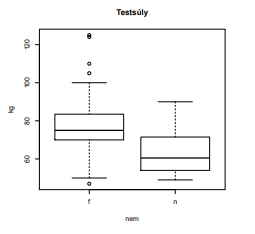
\includegraphics{boxplot}

\section{(172) Irja rá az ábrára, hogy melyik tanult eloszláscsalád sűrűségfüggvényeit mutatják be és
egészítse ki a jelmagyarázatot is.}

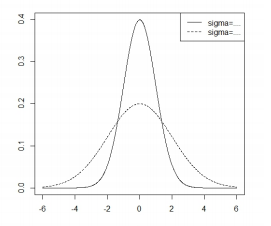
\includegraphics{fuggveny}

 Normális eloszlások (0 várható értékkel) a folytonos a standard, a szaggatott 2 szórású
(a sűrűségfüggvény képletét egybevetve az ábrával leolvasható)


\section{(173) Miért volt érdemes az alábbi módon alkalmazni a hist függvényt? Rajzolja fel a függvény eredményét! }

\begin{verbatim}
hist(diak[,7],xlab="jegy",ylab="gyakoriság",main="Analízis
jegy",breaks=c(1:6)-1/2)
\end{verbatim}

Azért jó ez az intervallum-beosztás, mert így pontosan középre esnek a tényleges értékek
és nem keletkeznek "üres" oszlopok, amik a default beállításnál előfordulhatnak.

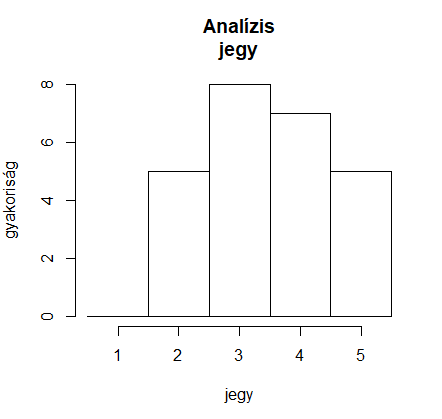
\includegraphics{histogram}

\section{(174)  Mit vizsgáltunk? Mit kaptunk eredményül? Mi p.v jelentése?}

\begin{verbatim}
p.v=rep(0,times=365);atlb=p.v;atlk=p.v
for (i in 1:365)
{jan1b<-homb[365*r+i,1];jan1k<-homk[365*r+i,1]
p.v[i]=t.test(jan1b,jan1k,paired=T,alternative="t")\$p.value
atlb[i]=mean(jan1b);atlk[i]=mean(jan1k)}
plot(p.v,type="l")
\end{verbatim}

p.v a p-értékek vektora az év napjaira. T-proba

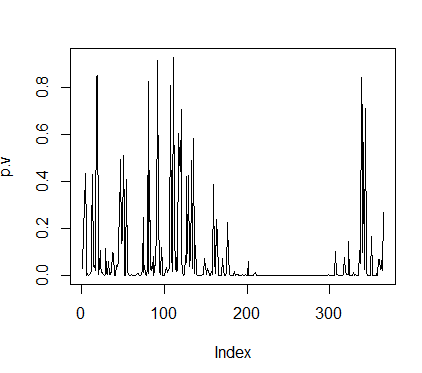
\includegraphics{pv}

\section{(175) Milyen görbe van az ábrán? Milyen valószínúségszámítási tulajdonságai vannak?}

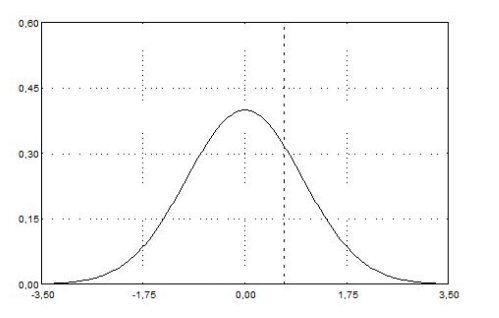
\includegraphics{gorbe}

ez standard normális eloszlás súrúségfüggvénye.


\section{(176) Mit vizsgáltunk? Mit ad meg a p? Egészítse ki a táblázatot a hiányzó értékekkel!}

\begin{verbatim}
n<-4;j<-6; q<-c(1:n)/n
h<-c(-Inf,qnorm(q)); mu<-mean(diak[,j])
sig=sd(diak[,j]) ; h<-h*sig+...
nu<-rep(0,times=n)
for (i in 1:n)
nu[i]<- sum((diak[,j]<h[i+1]) & (diak[,j]...h[i]))
np<-sum(nu)*rep(1/n,times=n)
c<-sum((nu-...)^2/np)
p<-1-pchisq(c,n-3)
\end{verbatim}

Lineáris modellt illesztettünk a
szeptemberi átlaghúmérsékletekre a nap sorszámának függvényében

A p a p-értéket jelöli.

Kiegészített változat:

\begin{verbatim}
n<-4;j<-6; q<-c(1:n)/n
h<-c(-Inf,qnorm(q)); mu<-mean(diak[,j])
sig=sd(diak[,j]) ; h<-h*sig+mu
nu<-rep(0,times=n)
for (i in 1:n)
nu[i]<- sum((diak[,j]<h[i+1]) & (diak[,j]>=h[i]))
np<-sum(nu)*rep(1/n,times=n)
c<-sum((nu-np)^2/np)
p<-1-pchisq(c,n-3)
\end{verbatim}

N jelentese a minták száma. $j$ a súly.


\section{(177) Milyen statisztikai fogalmat illusztrál az ábra? Milyen tulajdonságai vannak?}

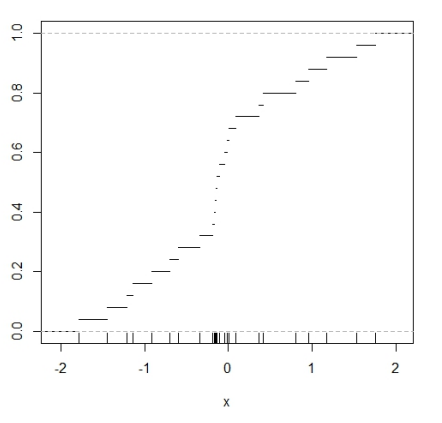
\includegraphics[scale=1.0]{gorbe2}

Ez standard normális eloszlású minta tapasztalati eloszlásfüggvénye.

\end{document}